\chapter{Exemplos}

Nesta seção serão apresentados os exemplos práticos escolhidos para o projeto e feitos com o auxílio do Jupyter Lab, ambiente de desenvolvimento do Python.

\section{Regressão Linear}

\subsection{O que é Regressão Linear?}
\label{sec:wifi}

Uma regressão linear nada mais é do que uma equação matemática utilizada para se estimar o valor de uma variável \(y\), dados os valores de algumas outras variáveis \(x\). Os modelos de regressão \textbf{simples} envolvem somente duas variáveis: uma independente \(x\) e uma dependente \(y\). Ela é chamada \textbf{linear} poque a relação entre os parâmetros se dá por uma \textbf{função linear} do tipo:

\[ \large F(x) = y = m \cdot x + c \]

Onde \(x\) é a variável independente, \(y\) é a variável dependente, \(m\) é o \textbf{coeficiente angular/declive} e \(c\) é o \textbf{coeficiente linear/intercepto}. O parâmetro \(c\) é o valor de \(F(x)\) quando \(x = 0\). O parâmetro \(m\) é a variação em \(F(x)\) quando variamos $x$ em 1 unidade.

O que pretendemos aqui é, a partir de um conjunto de dados $(x,y)$, obter um modelo linear de função $F(x) = y$ que relacione de modo mais exato possível a relação entre  as variáveis $x$ e $y$. Para que possamos entender a regressão linear em sua integridade, duas concepções são bastante importantes: a de \textbf{Função de Custo} e \textbf{Gradiente Descendente}. 

% \ref{fig:esp8266}.

%\begin{figure}[!htb]
%	\centering
%	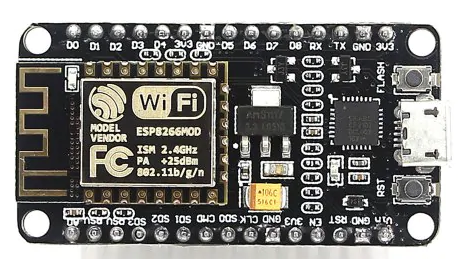
\includegraphics[width=0.4\textwidth]{./esp8266.png} 
%	\caption{Foto do módulo Wi-Fi ESP8266.}
%	\label{fig:esp8266}
%\end{figure}

\subsection{O que é Função de Custo?}
\label{sec:bt}

No contexto de otimização algorítmica, a função que queremos minimizar ou maximizar é denominada \textbf{função objetivo}. Quando queremos minimizá-la, ela é chamada \textbf{função de custo}. A função de custo computa a diferença entre o valor obtido em nosso modelo ($y_{modelo}$) e o valor real ($y_{real}$). \textbf{Entropia cruzada} e \textbf{Erro Quadrático Médio} são os tipos de funções de custo mais comuns. A fórmula para o Erro Quadrático Médio para $n$ amostras de dados é:

\[\large E=\frac{1}{n}\sum_{i=0}^{n}(y_{i,real} - y_{i,modelo})^{2} = \frac{1}{n}\sum_{i=0}^{n}(y_{i,real} - (m \cdot x_{i} + c))^{2}\]

Em sua essência, o conceito de função de custo é bastante simples: é um método para avaliar o quão bem o seu algoritmo modela o conjunto de dados em estudo. Se as predições estiverem totalmente erradas, a função de custo terá um valor maior. Se as predições estiverem corretas, a função de custo terá um valor menor. Na medida que mudados o nosso algoritmo, a função de custo irá nos dizer se estamos indo para o caminho correto.

\subsection{Gradiente Descendente}
Gradiente Descendente é um algoritmo de optimização usado para obter o mínimo de uma função diferenciável. Aqui, ela será utilizada para realizar o ajuste dos parâmetros $m$ e $c$ de forma iterativa com o objetivo de encontrar os valores para esses parâmetros que minimizem a função de custo o máximo possível. O Método do Gradiente se inicia atribuindo valores aleatórios para os parâmetros $m$ e $c$, valores estes que irão melhorar gradualmente a cada iteração, dando um pequeno passo de cada vez até que a função de custo convirja para um mínimo. O tamanho dos passos é definido por um parâmetro denominado \textbf{taxa de aprendizado}.

Na aplicação do Método do Gradiente, utilizamos as derivadas parciais da função de custo em relação a $m$ e em relação a $c$. O objetivo do método é, então, achar o mínimo global da função de custo a partir dessas derivadas parciais:

\[\large D_{m} = \frac{2}{n}\sum_{i=0}^{n}(y_{i,real} - (m \cdot x_{i} + c))\cdot(-x_{i}) = \frac{-2}{n}\sum_{i=0}^{n}(y_{i,real} - y_{i,modelo})\]

\[\large D_{c} = \frac{-2}{n}\sum_{i=0}^{n}(y_{i,real} - y_{i,modelo})\]

% \url{www.tablesgenerator.com}.

%\begin{table}[!htb]
%\centering
%\begin{tabular}{l|l|l}
%    ~       & ESP8266   & HC-05      \\
%    \hline
%    Alcance & 50m       & 10m        \\
%    \hline
%    Consumo & 170mA     & 40mA       \\
%    \hline
%    Preço   & R\$ 22,90 & R\$ 25,90  \\
%    \hline
%\end{tabular}
%\caption{Comparativo entre módulos ESP8266 e HC-05}
%\label{tab:semfio}
%\end{table}

\subsection{Regressão Linear por Gradiente Descendente no Python}
Vamos modelar uma função $F(x)$ para um conjuntos de dados armazenados em um arquivo csv, utilizando o Erro Quadrático Médio e o Gradiente Descendente.

Primeiramente, vamos plotar o gráfico de dispersão das amostras para se ter uma ideia inicial da distribuição dos dados. Usaremos o conjunto de dados armazenados neste link:
\url {https://github.com/Joe-Taka/REA/blob/main/C%C3%B3digos/Exemplo%201%20-%20Regress%C3%A3o%20Linear/data.csv}

\begin{minted}{python}
	import numpy as np
	import pandas as pd
	import matplotlib.pyplot as plt
	# Definindo um tamanho para a figura
	plt.figure(figsize=(7,6))
	# Pegando os valores do arquivo 'csv'
	data = pd.read_csv('data.csv')
	# Pegando a 1° coluna
	X = data.iloc[:, 0]
	# Pegando a 2° coluna
	Y = data.iloc[:, 1]
	# Gráfico de dispersão para as amostras
	plt.scatter(X, Y)
	plt.show()
\end{minted}

\begin{figure}[H]
	\centering
	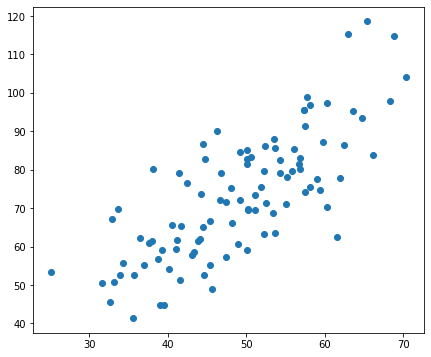
\includegraphics[width=0.6\textwidth]{./Imagens/Regressão Linear/RL1.png} 
	\caption{Gráfico de dispersão}
	\label{fig:RL1}
\end{figure}

Aplicando o \textbf{Gradiente Descendente}: começamos atribuindo valores nulos para os parâmetros $m$ e $c$ e iteramos as derivadas parciais da função de custo mil vezes, até encontrar os valores ótimos para os parâmetros:

\begin{minted}{python}
# Suposições iniciais para os parâmetros
m = 0
c = 0
plt.figure(figsize=(7,6))
# Taxa de aprendizado
L = 0.0001  
# Número de iterações para o Gradiente Descendente
epochs = 1000  
n = float(len(X)) # Número de elementos de X
# Aplicando a iteração do Método Gradiente 
for i in range(epochs): 
	Y_pred = m*X + c  # Valor atual suposto para Y
	D_m = (-2/n) * sum(X * (Y - Y_pred)) 
	D_c = (-2/n) * sum(Y - Y_pred) 
	m = m - L * D_m  # Atualizando m
	c = c - L * D_c  # Atualizando c
print (f"Valor para m: {m:.2f}; Valor para c: {c:.2f}")
# Valor para m: 1.48; Valor para c: 0.10
Y_pred = m*X + c
plt.scatter(X, Y) 
plt.plot([min(X), max(X)], [min(Y_pred), 
max(Y_pred)], color='red')
plt.show()
\end{minted}

\begin{figure}[H]
	\centering
	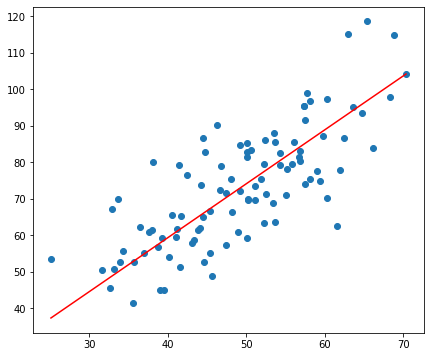
\includegraphics[width=0.6\textwidth]{./Imagens/Regressão Linear/RL2.png} 
	\caption{Regressão Linear}
	\label{fig:RL2}
\end{figure}

Para o conjunto de dados fornecidos em nosso exemplo, a função do nosso modelo fica, então:

\[ \large F(x) = 1,48 \cdot x + 0,10 \]

\subsection{Aplicações da Regressão Linear}

\begin{itemize}
\item Aprendizado de máquina, como uma ferramenta de predição.
\item Em modelo de negócios, pode ser utilizado para gerar insights à respeito do comportamento do consumidor, de modo a entender os fatores que possam influenciar na lucratividade do negócio. Por exemplo, se as vendas de uma empresa aumentaram constantemente todos os meses nos últimos anos, ao se realizar uma análise linear dos dados de vendas com as vendas mensais, a empresa é capaz de prever as vendas nos meses futuros. 
\item Química analítica, principalmente na calibração de dados para gerar as chamadas \textbf{curvas de calibração}.
\item Nas ciências dos materiais, como uma forma de prever as propriedades de certos materiais.
\item Em finanças, como uma ferramenta para traçar as curvas de tendências de ativos.

\end{itemize} 



